\documentclass[11pt]{article}

\usepackage{fancyhdr}
\usepackage{graphicx}
\usepackage{geometry}
\usepackage{lastpage}
\usepackage{titling}
\usepackage{sectsty}
\usepackage{setspace}
\usepackage{changepage}
\usepackage[shortlabels]{enumitem}
\usepackage{subcaption}
\usepackage{helvet}
\usepackage{hyperref}
\usepackage{tabularx}

\usepackage{siunitx}
\usepackage{nicefrac}
\usepackage{amsmath}
\usepackage{gensymb}
\usepackage{amssymb}
\usepackage{float}

\usepackage{listings}
\usepackage{color}
\definecolor{dkgreen}{rgb}{0,0.6,0}
\definecolor{gray}{rgb}{0.5,0.5,0.5}
\definecolor{mauve}{rgb}{0.58,0,0.82}

\lstset
{
  frame=tb,
  language=MATLAB,
  aboveskip=3mm,
  belowskip=3mm,
  showstringspaces=false,
  columns=flexible,
  basicstyle={\small\ttfamily},
  numbers=none,
  numberstyle=\tiny\color{gray},
  keywordstyle=\color{blue},
  commentstyle=\color{dkgreen},
  stringstyle=\color{mauve},
  breaklines=true,
  breakatwhitespace=true,
  tabsize=3
}

\geometry
{
  letterpaper, 
  total={175.9mm,229.4mm}, 
  top=25mm, 
  left=20mm, 
  headheight=15pt,
  voffset=12pt,
  footskip=15pt
}
\author{Daniel Sturdivant}
\title{Homework 2}
\date{February 2023}
\graphicspath{ {./media/} }

\pagestyle{fancy}
\fancyhead[R]{February 13, 2023}
\fancyhead[L]{Sturdivant, Daniel}
\fancyhead[C]{MECH 6970 Intro to GPS}
\fancyfoot[C]{Page \thepage\ of \pageref{LastPage}}

\makeatletter
\def\@maketitle
{
  \null
  \begin{center}
    {\huge \@title \\}
  \end{center}
  \vskip 5mm
}
\makeatother

\sectionfont{\fontsize{16}{16}}
\subsectionfont{\fontsize{13}{13}\normalfont}
\renewcommand{\thesubsection}{\arabic{section}-\arabic{subsection}}
\renewcommand{\familydefault}{\sfdefault}
\newcommand{\solution}{\textbf{Solution: \\}}


%% ====================================================================== %%
\begin{document}

\maketitle
\thispagestyle{fancy}
\setstretch{1.25}
% \setlength{\parskip}{0em}
% \setlength{\abovedisplayskip}{-8pt}
% \setlength{\belowdisplayskip}{12pt}
\setlength{\parindent}{0pt}

\begin{enumerate}[label=\textbf{\arabic*.}]
  \itemsep 24pt
  \item Consider a simple estimation of a single parameter: $y=a$, where the 
  measurement noise has unit variance.
  \begin{enumerate}[(a)]
    \itemsep -2pt
    \item Determine the accuracy of the parameter estimate as a function of 
    the number of measurements.
    \item Verify the results through a monte-carlo simulation.
  \end{enumerate}
  \solution
  The variance on any given measurement can be defined with expectation as:
  \begin{equation*}
    \sigma^2 = E\{(y-\bar{y})(y-\bar{y})\} = \sigma^2
  \end{equation*}
  With more measurements at the same point, the variance decreases as follows:
  \begin{equation}
    \sigma_M^2 = \dfrac{\sigma^2}{M}
  \end{equation}
  Where $M$ is the number of measurements. Taking the square root of 
  \emph{equation 1} provides the standard deviation which is in the same units as 
  the measurement. To confirm this with a monte-carlo simulation, a simple 
  simulation with on a measurement of $y=1$ is performed. A total of 1-500 
  measurements were simulated for each of 1000 monte-carlo runs. Below is 
  a plot of the results:
  \begin{figure}[H]
    \centering
    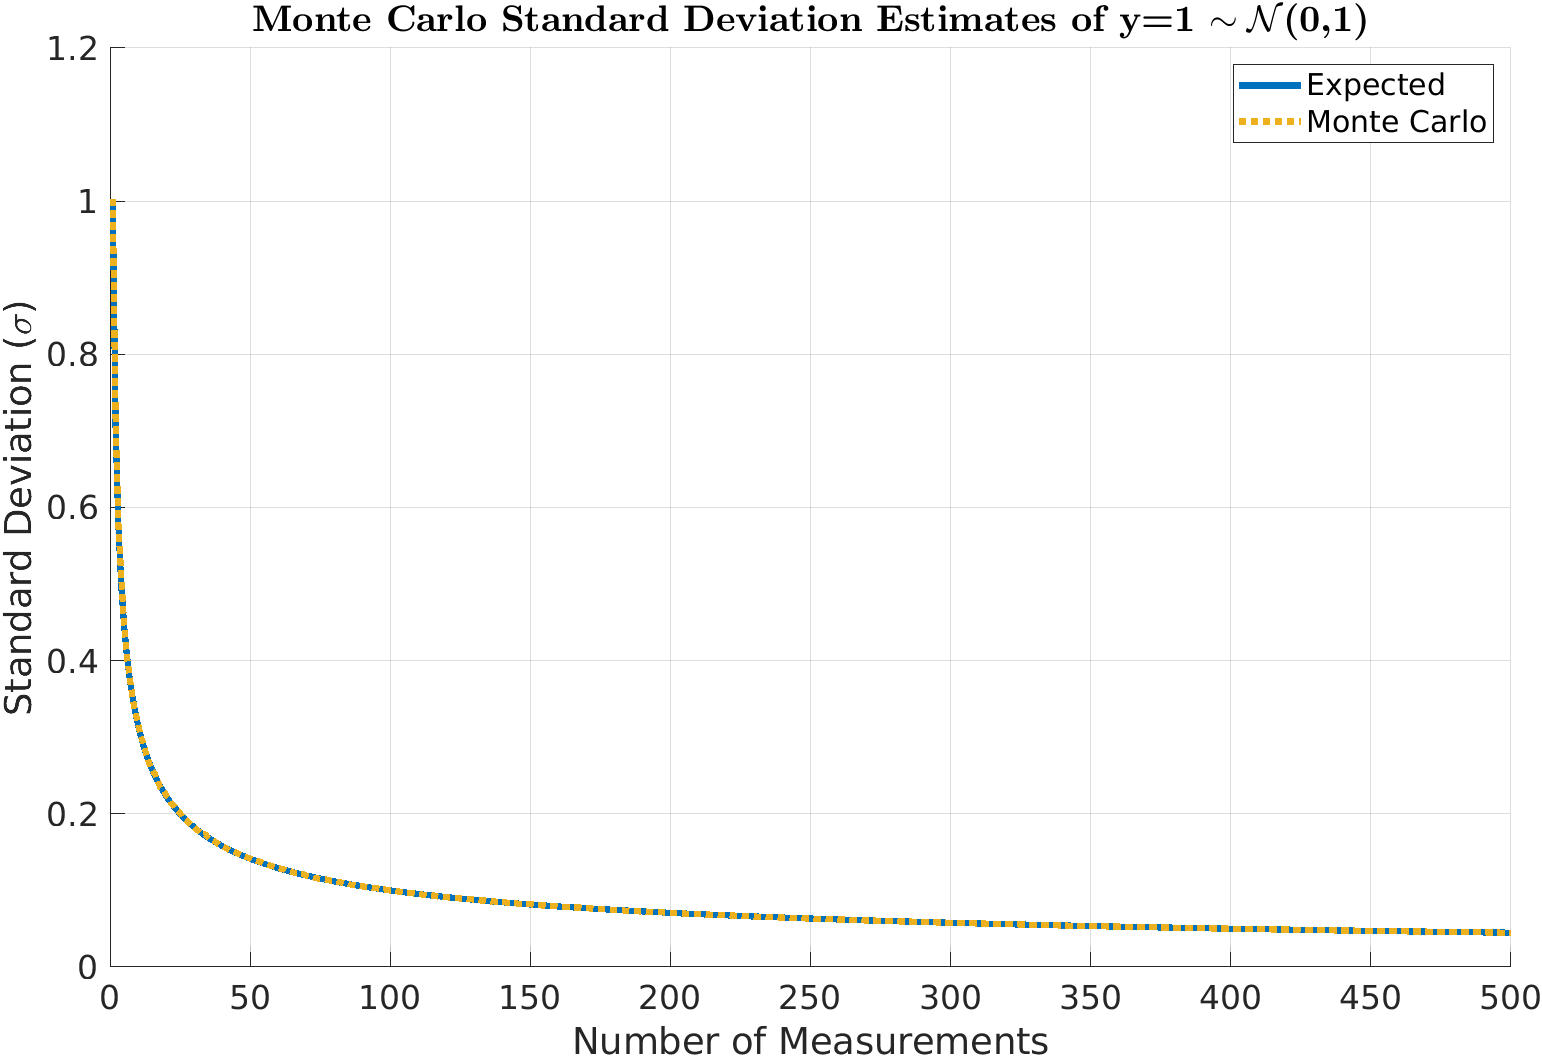
\includegraphics[width=0.7\textwidth]{p1.png}
    \caption{Effect of the Number of Measurements on Accuracy}
  \end{figure}

  \item Given the set of data, perform a least-squares fit to solve for the 
  model coefficients and the predicted estimation error (1-$\sigma$) for the 
  coefficient \emph{a} assuming the 1-$\sigma$ measurement noise on y is 0.4.
  \begin{center}
    \begin{tabularx}{0.8\textwidth} { 
      | >{\centering\arraybackslash}X 
      | >{\centering\arraybackslash}X 
      | >{\centering\arraybackslash}X 
      | >{\centering\arraybackslash}X 
      | >{\centering\arraybackslash}X 
      | >{\centering\arraybackslash}X | }
      \hline $x$ & 0 & 1 & 2 & 3 & 4 \\
      \hline $y$ & 0.181 & 2.680 & 3.467 & 3.101 & 3.437 \\
      \hline
    \end{tabularx}
  \end{center}
  \begin{enumerate}[(a)]
    \itemsep -2pt
    \item $y = a + bx$
    \item $y = a + bx + cx^2$
    \item $y = a + bx + cx^2 + dx^3$
    \item Is the estimate for $a$ consistent? Why or why not? Which is probably 
    the correct prediction of the estimation error on $a$?
  \end{enumerate}
  \solution
  Defining the observation matrix for each part (subscript defining part):
  \begin{equation*}
    \begin{split}
      H_a &= \begin{bmatrix} 1 & x \end{bmatrix} \\
      H_b &= \begin{bmatrix} 1 & x & x^2 \end{bmatrix} \\
      H_c &= \begin{bmatrix} 1 & x & x^2 & x^3 \end{bmatrix}
    \end{split}
  \end{equation*}
  With the measurement vector ($y$) being the defined in the table and estimating 
  the coefficients in each part with the least squares formula below, the estimate 
  of $a$ is as follows:
  \begin{equation*}
    x = (H^T H)^{-1}H^T y
  \end{equation*}
  \begin{equation*}
    \begin{split}
      a_a &= 1.186 \\
      a_b &= 0.404 \\
      a_c &= 0.126
    \end{split}
  \end{equation*}
  This estimate is not consistent. Looking at the standard deviation on each 
  estimate of $a$:
  \begin{equation*}
    \begin{split}
      \sigma_{a_a} &= 0.310 \\
      \sigma_{a_b} &= 0.376 \\
      \sigma_{a_b} &= 0.397
    \end{split}
  \end{equation*}
  It appears that the linear estimate of $a$ is the most accurate. This is likely 
  due to the fact that the additional higher order terms dominate the overall 
  curve fit as well as not including measurement noise in the higher order models. 
  However, looking at the plot below, it is clear that a third order approximation 
  provides the best fit.
  \begin{figure}[H]
    \centering
    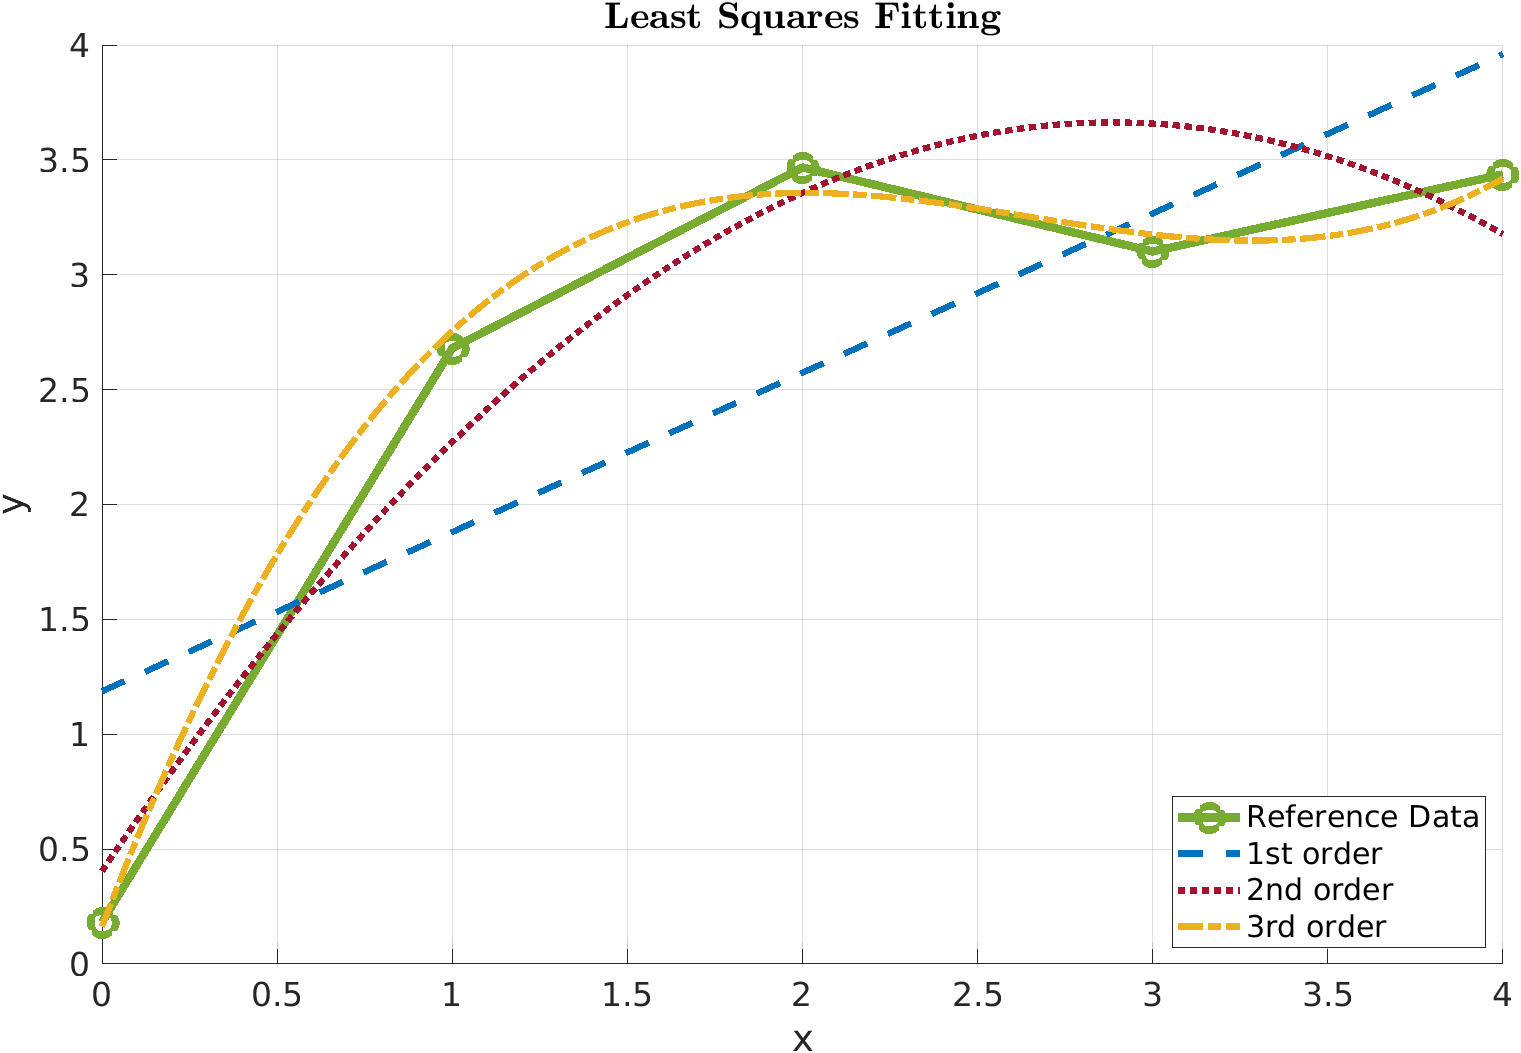
\includegraphics[width=0.7\textwidth]{p2.png}
    \caption{Curve Fit Coefficient Matching}
  \end{figure}

  \item Given the following range equation $r^2 = (x-a)^2 + (y-b)^2$ with a 
  range error of 0.5 meters (1-$\sigma$) and the table below:
  \begin{center}
    \begin{tabularx}{0.8\textwidth} { 
      | >{\centering\arraybackslash}X 
      | >{\centering\arraybackslash}X 
      | >{\centering\arraybackslash}X 
      | >{\centering\arraybackslash}X 
      | >{\centering\arraybackslash}X | }
      \hline $a$ & 0 & 10 & 0 & 10 \\
      \hline $b$ & 0 & 0 & 10 & 10 \\
      \hline $r^2$ & 25 & 65 & 45 & 85 \\
      \hline
    \end{tabularx}
  \end{center}
  \begin{enumerate}[(a)]
    \itemsep -2pt
    \item Find the Jacobian Matrix.
    \item What is the expected solution uncertainty?
    \item What is the solution for $x$ and $y$?
    \item Perform a monte-carlo simulation and verify \emph{part b}.
  \end{enumerate}
  \solution
  Given this equation is linear for $r^2$, the Jacobian can be easily made by 
  taking the partial derivatives of $r^2$ with respect to $x$ and $y$.
  \begin{equation*}
    \begin{split}
      \dfrac{\partial r^2}{\partial x} &= 2(x-a) \\
      \dfrac{\partial r^2}{\partial y} &= 2(y-b)
    \end{split}
  \end{equation*}
  Applying a taylor series expansion:
  \begin{equation*}
    r^2 = (x_0 - a)^2 + (y_0 - b)^2 + 2(x_0-a)\Delta x + 2(y_0-b)\Delta y
  \end{equation*}
  Creating the Jacobian by plugging in $a$ and $b$:
  \begin{equation*}
    H = 
    \begin{bmatrix}
      2(x_0 - 0) & 2(y_0 - 0) \\
      2(x_0 - 10) & 2(y_0 - 0) \\
      2(x_0 - 0) & 2(y_0 - 10) \\
      2(x_0 - 10) & 2(y_0 - 10) \\
    \end{bmatrix}
  \end{equation*}
  And the following system:
  \begin{equation*}
    \begin{split}
      y &= Hx \\
      \begin{bmatrix}
        \Delta x \\ \Delta y
      \end{bmatrix}
      &=
      \begin{bmatrix}
        2(x_0 - 0) & 2(y_0 - 0) \\
        2(x_0 - 10) & 2(y_0 - 0) \\
        2(x_0 - 0) & 2(y_0 - 10) \\
        2(x_0 - 10) & 2(y_0 - 10) \\
      \end{bmatrix}
      \begin{bmatrix}
        25 - ((x_0 - 0)^2 + (y_0 - 0)^2) \\
        65 - ((x_0 - 10)^2 + (y_0 - 0)^2) \\
        45 - ((x_0 - 0)^2 + (y_0 - 10)^2) \\
        85 - ((x_0 - 10)^2 + (y_0 - 10)^2) \\
      \end{bmatrix}
    \end{split}
  \end{equation*}
  Initializing at $\begin{bmatrix} 0 & 0 \end{bmatrix}^T$ and using Newton-Raphson 
  to iteratively solve the problem, the solution and expected uncertainty are:
  \begin{equation*}
    \begin{split}
      \begin{bmatrix}
        x \\ y
      \end{bmatrix}
      &=
      \begin{bmatrix}
        3 \\ 4
      \end{bmatrix}
      \si{m}
      \\
      \sigma_x &= 0.0232 \:\si{m}\\
      \sigma_y &= 0.0246 \:\si{m}
    \end{split}
  \end{equation*}
  Performing a monte-carlo of 1000 iterations results in a simulation standard 
  deviation of:
  \begin{equation*}
    \begin{split}
      \sigma_x &= 0.0230 \:\si{m}\\
      \sigma_y &= 0.0250 \:\si{m}
    \end{split}
  \end{equation*}
  Which matches very closely to the expected value.

  \item Using the provided data file containing GPS and SOOP satellites along 
  with their simulated psuedoranges and a 1-$\sigma$ accuracy of 0.5 meters:
  \begin{enumerate}[(a)]
    \item Calculate the position and expected horizontal and vertical error using 
    the first 4 GPS satellites, initialized at the center of the earth. How 
    many iterations does it take?
    \item Repeat \emph{part a} with all 9 satellites.
    \item Repeat \emph{part a} assuming a perfect clock.
    \item Calculate the position using 2 GPS and SOOP satellites. What happens 
    and why?
    \item Repeat \emph{part c} with an initial condition of 
    $[423000, -5362000, 3417000]$.
  \end{enumerate}
  \solution
  Using the psuedorange geometry matrix defined in class:
  \begin{equation*}
    G = 
    \begin{bmatrix}
      \dfrac{-u_x}{r} & \dfrac{-u_y}{r} & \dfrac{-u_z}{r} & 1
    \end{bmatrix}
  \end{equation*}
  \begin{center}
    \captionof{table}{Parts a-e solution}
    \begin{tabularx}{0.8\textwidth} { 
      | >{\centering\arraybackslash}X 
      | >{\centering\arraybackslash}X 
      | >{\centering\arraybackslash}X 
      | >{\centering\arraybackslash}X 
      | >{\centering\arraybackslash}X 
      | >{\centering\arraybackslash}X | }
      \hline            & \textbf{\# SV} & \textbf{\# SOOP} & \textbf{Iterations} & \textbf{HDOP} & \textbf{VDOP}  \\
      \hline \textbf{a} & 4              & 0                & 5                   & 7.403         & 8.307 \\
      \hline \textbf{b} & 9              & 0                & 5                   & 0.977         & 1.086 \\
      \hline \textbf{c} & 4              & 0                & 5                   & 7.403         & 8.307 \\
      \hline \textbf{d} & 2              & 2                & N/A                 & N/A           & N/A   \\
      \hline \textbf{e} & 9              & 0                & 3                   & 0.977         & 1.086 \\
      \hline
    \end{tabularx}
  \end{center}
  The data when utilizing the SOOP satellites in combination with the GPS satellites 
  is unavailable because the SOOP satellites cause the geometry matrix to be poorly 
  conditioned. This causes the user position to be unobservable since the number 
  of usable measurements is fewer than 4.

  \item The ionosphere (50-1000 km above the Earth) is one source of error on GPS 
  psuedoranges. Ionospheric delay is a function of how much atmosphere the signal 
  passes through, which is a function of the elevation angle, $\theta$. A simple 
  model is as follows:
  \begin{equation*}
    I(\theta) = A_1(1+16(0.53-\dfrac{\theta}{180})^3)
  \end{equation*}
  Where $A_1 = 5(10^{-9})$ seconds and $\theta$ is in degrees. Elevation masks, 
  a constant angle below which all signals are ignored, combat the significant 
  delays at low elevation angles.
  \begin{figure}[H]
    \centering
    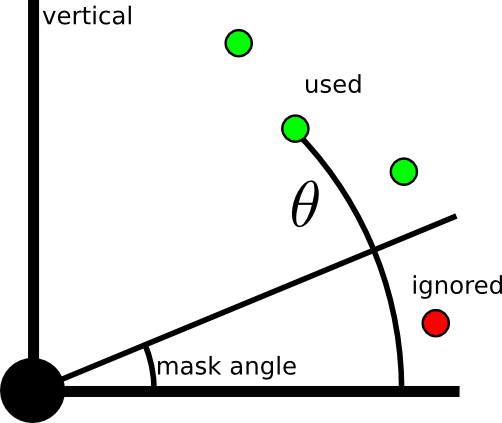
\includegraphics[width=0.4\textwidth]{q5.png}
  \end{figure}
  Using the 9 GPS satellite positions in the data file and the Ionospheric 
  delay model, generate a plot of position accuracy versus mask angle. Comment 
  on this plot. \\
  \solution
  Iterating through elevation angles starting at 0 degrees and ending when there 
  is fewer than 4 satellites in view creates the following plot:
  \begin{figure}[H]
    \centering
    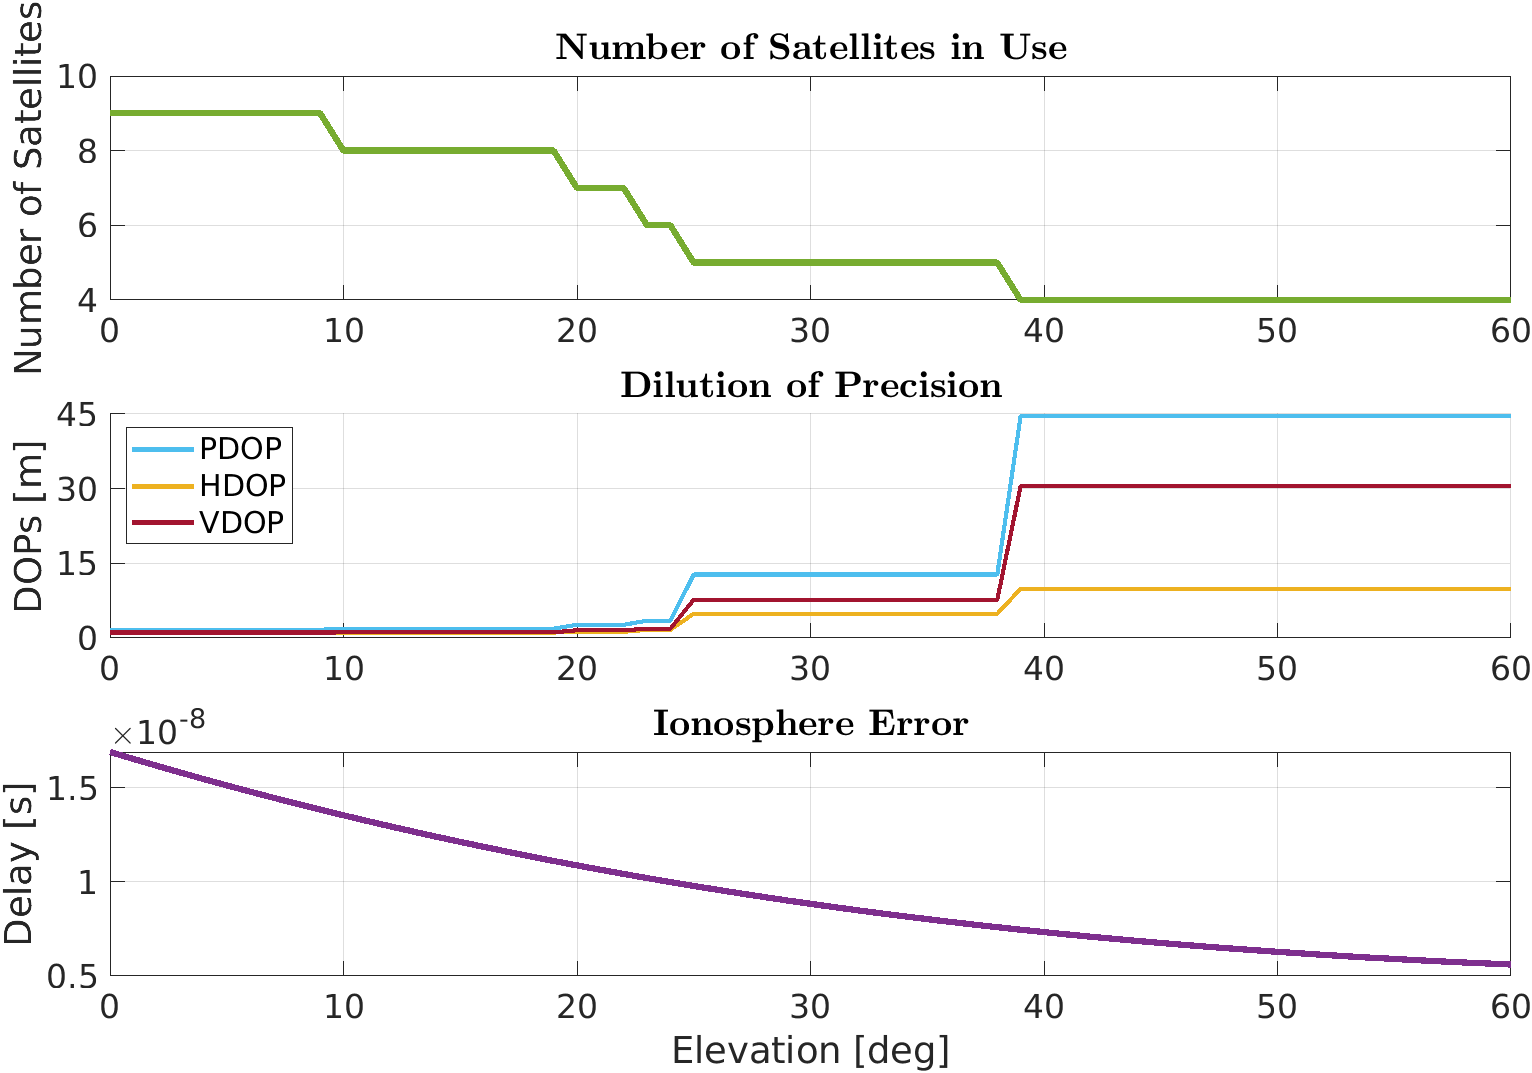
\includegraphics[width=0.95\textwidth]{p5.png}
    \caption{Errors when Increasing the Elevation Mask Angle}
  \end{figure}
  As shown, the positioning error increases as the elevation mask is increased, 
  particularly in the vertical direction. This is due to the reduced observability 
  as the satellites at lower elevations (closer to tangent with the higher 
  elevation satellites) get removed. The ionosphere error also decreases as the 
  elevation mask increases because less of the ionosphere is traversed by the 
  signal.
  
\end{enumerate}

\end{document}